%----------------------------------------------------------------------------------------
% PACKAGES AND OTHER DOCUMENT CONFIGURATIONS
% WARNING: Don't mess with any of the following unless you know what you are doing.
%----------------------------------------------------------------------------------------
\documentclass[english,12pt,a4paper,openany]{book}
\usepackage{datetime}
\usepackage{tabularx}
\usepackage{makecell}
\usepackage{eurosym}
\usepackage{pbox}
\usepackage[utf8]{inputenc}
\usepackage[T1]{fontenc}
\usepackage[english]{babel}
\usepackage{amsmath}
\usepackage{amsfonts}
\usepackage{fancyhdr}
\usepackage{amssymb}
\usepackage[dvipsnames]{xcolor}
\usepackage{mdframed}
\usepackage{multirow}
\usepackage{multicol} 
\usepackage{tikz}
\usepackage{graphicx}
\usepackage[absolute]{textpos} 
\usepackage{colortbl}
\usepackage{array}
\usepackage{geometry}
\usepackage{hyperref}
\pagestyle{fancy}
\renewcommand\headrulewidth{1pt}
\usepackage{float}
\usepackage{dirtree}

%------------------------------------------------------------------------------------------------------
%	The following are the RGB values for the official ATU colours.
%------------------------------------------------------------------------------------------------------	
\definecolor{ATUGreen}{RGB}{0, 91, 94}
\definecolor{ATULightGreen}{RGB}{172, 245, 189}
\definecolor{ATUNavy}{RGB}{0, 26, 121}
\definecolor{ATUOrange}{RGB}{255, 121, 30}
\definecolor{ATUPurple}{RGB}{77, 8, 87}
\definecolor{ATUSand}{RGB}{255, 232, 212}
\definecolor{ATUTeal}{RGB}{123, 185, 203}
\definecolor{ATUWarmGrey}{RGB}{200, 190, 191}
\definecolor{ATUYellow}{RGB}{248, 255, 142}



%------------------------------------------------------------------------------------------------------
%	******* CHANGE THE FOLLOWING VARIABLES
%------------------------------------------------------------------------------------------------------	

\newcommand{\reportauthor}{GABRIEL HANG} % Change to your name
\newcommand{\projecttitle}{Streamlining CI/CD Pipeline into Web Development}
\newcommand{\reporttype}{Minor Dissertation} %Report  type (Project Plan / Final Report)
\newcommand{\supervisorname}{JOSEPH CORR} %Report  type (Project Plan / Final Report)
\newdateformat{monthyeardate}{\monthname[\THEMONTH], \THEYEAR}





%------------------------------------------------------------------------------------------------------	
% WARNING: Don't mess with any of the following unless you know what you are doing.
%------------------------------------------------------------------------------------------------------	
\pagestyle{fancy}
\fancyhf{}
\fancyhead[R]{\textcolor{ATUGreen}{\reportauthor}}
\fancyhead[L]{\textcolor{ATUGreen}{\projecttitle}}
\fancyfoot[L]{\textcolor{ATUGreen}{Atlantic Technological University (ATU), Galway.}}
\fancyfoot[R]{\thepage}

\begin{document}
\begin{titlepage}

\newgeometry{left=6cm,bottom=2cm, top=1cm, right=1cm}

\tikz[remember picture,overlay] \node[opacity=1,inner sep=0pt] at (2.2mm,-165mm){
\includegraphics{images/leftbar.png}}; % Fond changeable 

\fontfamily{fvs}\fontseries{m}\selectfont
\color{white}

\begin{picture}(0,0)
\put(-110,-743){\rotatebox{90}{\Huge{B.Sc. (Hons) in Software Development}}}
\end{picture}
 
\vspace{-10mm} 

\flushright 
\includegraphics[width=100mm]{images/atu-logo-green.png} 

\flushright
\vspace{10mm}
\textcolor{ATUGreen}{
\fontfamily{cmss}\fontseries{m}\fontsize{22}{26}\selectfont
\projecttitle
}
\normalsize
\color{black}

\vspace{1.5cm}
\normalsize
\textbf{By \\ \textcolor{ATUGreen}{\reportauthor}}\\ %Dr. John Healy
\vspace{15mm}
\textbf{for \\  \supervisorname}\\
\vspace{15mm}
{\scshape \today} \\[0.3\baselineskip]
\vspace{75mm}
\Large {\textcolor{ATUGreen}{\textbf{{\reporttype}}}} \\
\bigskip
\normalsize
\textbf{Department of Computer Science \& Applied Physics,\\School of Science \& Computing,\\Atlantic Technological University (ATU), Galway.}\\
\end{titlepage}
\newpage
\tableofcontents
\listoffigures
\listoftables
\pagenumbering{arabic} 

%----------------------------------------------------------------------------------------
%	   ******* CHANGE the Chapters if necessary. Each chapter is encapsulated inside 
%                 its own file. The chapters below are based on the guidelines 
%                 given in the lecture.
%----------------------------------------------------------------------------------------
\chapter{Introduction}

In today's rapidly advancing digital era, the importance of software development has increased significantly, with businesses relying heavily on applications to meet the demands of their customers \cite{hf}. However, developing software is a complex process, and with the ever-increasing need for faster and more reliable software delivery, traditional development methods are no longer sufficient \cite{dsmgm}. As software development processes can involve multiple stages, it takes a significant amount of time and effort to complete. Moreover, developers may be tasked with multiple projects simultaneously, which can result in further delays. As such, this can lead to customer dissatisfaction and lost opportunities \cite{sb}.

Automation has emerged as a solution to tackle the problem of slow software development delivery. It improves both the time and cost effectiveness of software development by allowing software development teams to allocation resources more efficiently. For instance, Automation can help with tasks that require creative thinking or technical expertise, such as system integration, feature design, and debugging. Furthermore, automation reduces the time required to complete repetitive and mundane tasks, lowering operational costs. Automation, whether partially or fully implemented, can significantly improve software development processes \cite{saarenpaa2020creating}.

Continuous integration and continuous deployment (CI/CD) development practices have become increasingly popular for productivity and efficiency in recent years. Despite its growing popularity, some may argue that setting up CI/CD is time consuming and complex \cite{sander}. Therefore, it is vital to study and research this topic to ensure that development teams can effectively implement and reap the benefits of CI/CD.

\section{Background Information}

Continuous integration and continuous deployment have become crucial components for efficient and effective software delivery. In a survey conducted by a software testing company, Mabl, about half of the 500 participants are implementing CI, and a quarter are going to implement it in the near future. Conversely, 190 respondents out of 500 use CD while another 150 respondents planning to implement it \cite{clark}. 

By streamlining the CI/CD pipeline, developers can automate testing, deployment, and delivery processes, thereby reducing the risk of errors and ensuring faster release cycles \cite{kubinyi}. These practices help developers automate the process of building, testing, and deploying their applications, allowing them to deliver software updates more quickly and efficiently. This approach can also improve collaboration among development teams, operations, and other stakeholders, ultimately leading to better software quality and user satisfaction \cite{bs}.

\section{Problem Statement}
According to multiple studies \cite{sb, saarenpaa2020creating, saz, chen, dm, phillips2015manager}, CI/CD pipelines enable the quick and dependable delivery of software changes, making it possible to implement new or amended product and service features within a shorter time frame. This significantly reduces the time required to implement ideas or fixes from weeks or months to a matter of days. This has shown that CI/CD pipelines have a positive impact on software development process.

However, it is true that setting up the pipelines can be difficult especially for those who are new to it or want to integrate an existing project \cite{sander}. Hence, it is crucial to have the be prepared to acknowledge the challenges that come during implementation as it requires a deep understanding of the development environment, structure and tools involved.

In response to the problem, the purpose of this research paper is to study and examine the CI/CD pipeline while designing a web application to test and deploy.

\section{Significance of the Study}
The outcome of this project can help organizations to benefit greatly from the adoption of CI/CD pipelines. Organisations can accelerate the development and delivery of software features by automating the process of testing and deploying software. This can result in a shorter time-to-market, increased productivity, and a better overall for customers experience \cite{hf}.

Thus, clients or customers can receive more and faster feedback, as well as higher quality software as developers can detect and fix bugs earlier in the development cycle With CI/CD pipelines. Customers can also benefit from a more responsive and dynamic product with the ability to deploy new features and updates more frequently. \cite{chen, leppanenetal}.

Finally, this research can help the researcher and other learners to gain a deeper understanding of CI/CD principles. Teams can achieve a more efficient workflow, better collaboration, and higher code quality by automating the software development process, all of which are critical for project success \cite{sander}. In this context, for instance, a website has been developed and implemented with a CI/CD pipeline to better understand everything from the ground up.

\section{Objectives}
\begin{enumerate}
  \item To demonstrate an understanding of principles and practices of continuous integration and deployment for better efficiency.
  \item To enhance designing and developing a scalable web application using modern front-end frameworks and back-end technologies.
  \item To implement best practices for software development, such as testing and documentation.
  \item To develop skills in project management, including project planning and tracking.
\end{enumerate}

\section{Project Repository Overview and Key Components}
In this dissertation, the design and implementation of a CI/CD pipeline using GitHub Actions, while also developing a simple student grade management website using MERN stack with basic CRUD functionalities. The website is built using React.js as the front-end and MongoDB as the database, with Node.js and Express.js serving as the back-end server.

A functioning student grade management website that incorporates basic CRUD functionalities and demonstrates continuous integration and deployment principles and practices has been designed. The code for this project is hosted on GitHub, and can be found \href{https://github.com/gabhang/final-year-project}{here}. The website is built using React.js as the front-end and MongoDB as the database. Initially, the back-end server was developed in Go language, but it was later changed to Node.js and Express.js due to deployment compatibility and issues. Next, Jest and Supertest were used to write tests for testing, and Heroku was used for deployment. Lastly, Jira, a project management software, is utilised to plan and track project progress.

The student grade system deployed from this repository can be accessed \href{https://student-grade-system.herokuapp.com/}{here} and the following directory layout shows the hierarchy of directories and files for the project with description:\newline

\dirtree{%
.1 student-grade-system.
.2 .github/workflows.
.3 checks.yml.
.2 BACKEND.
.3 server.js.
.2 dissertation.
.2 public.
.2 src.
.3 components.
.4 create.SG.js.
.4 listings.js.
.4 updateSG.js.
.3 App.js.
.3 App.css.
.2 test.
.3 crud.test.js.
.2 .gitignore.
.2 Procfile.
.2 README.md.
.2 package-lock.json.
.2 package.json.
}

\begin{itemize}
\item .github/workflows/checks.yml: This file sets up GitHub Actions to run checks on each push request to ensure that the code passes all tests and deploys automatically to Heroku.
\item BACKEND/server.js: This file contains the back-end code for the project, which handles CRUD API requests and database interactions.
\item dissertation: This directory contains the author's dissertation in LaTeX format.
\item public: This directory contains public files, such as images and static HTML files.
\item src: This directory contains the main React source code for the project, including the components sub-directory that contains different pages of the website. The App.js file provides a navigation bar for every page, while the App.css file manages the CSS styles for the website.
\item tests/crud.test.js: This file contains tests for the project, testing the Create, Read, Update, and Delete (CRUD) functionality.
\item .gitignore: This file specifies files and directories to be ignored by Git when committing changes. For this project, the node\_modules and build folders are ignored, for instance.
\item Procfile: This file is used by Heroku to specify the commands to run when the app is deployed. In this project, this file is used to start the server.
\item README.md: This file provides an overview of the project.
\item package-lock.json: This file specifies version numbers for dependencies to ensure consistency across installations.
\item package.json: This file specifies the project's dependencies and scripts for running the app.
\end{itemize}
\chapter{Methodology}

The focus of this project is to design and implement a continuous integration and continuous delivery (CI/CD) pipeline. The pipeline would automate the building, testing, and deployment of the application to a production environment. In addition, a MERN (MongoDB, Express, React, Node.js) website is designed to integrate and test the pipeline automatically. The decision to carry out a CI/CD pipeline project was made due to the increasing popularity of automation in software development.

The project started with Agile development methodologies and transitioned to DevOps methodologies after completing the design and implementation of the CI/CD pipeline. Initially, the developer decided to switch the web application's backend from Node.js and Express.js to GO to make the project more challenging and the learn a new programming language. Basically, the idea was to build a pipeline and a website while pick up a new language.

Throughout the coding process, secondary resources were used frequently to learn GO and set up the workflow. After the website was fully designed and the features were fully implemented, the developer started designing the CI/CD pipeline. The CI part went smoothly as expected, but the CD part encountered some difficulties. The section on system evaluation will provide explanations and evidence. After attempting several solutions, the developer decided to switch back to the initial MERN stack as the focus was on designing the CI/CD pipeline.

This section will be divided into two parts: software development approaches and tools and technologies used in this project.

\section{Software Development Approaches}

The developer used Agile development methodologies initially for designing the website and the pipeline, and then transitioned to DevOps after completing the design and implementation of the CI/CD pipeline. However, it is important to note that DevOps is not limited to only CI/CD but is a combination of development and operations practices that emphasize automation and monitoring throughout the software development lifecycle.

By combining Agile development with DevOps practices, the developer aimed to create an efficient, reliable, and scalable software development process \cite{hlrf}. Agile provided flexibility and adaptation to changing requirements during the design and development phases, while DevOps ensured automation, testing, and monitoring during deployment and production phases. The integration of these two methodologies aimed to create a seamless and streamlined software development process from conception to production.

\subsection{Agile Development}
Moving away from traditional software development methodologies that are incapable of adapting to changes, the developer chose to use the agile method for the development phase as the project involves incremental changes and iterations and does not have fixed features as they may change due to factors such as time constraints. Furthermore, Agile methods strive for a faster release schedule, making them ideal for projects that require quick adaptability to changes \cite{aaa, hlrf, dragos, koch}. Table~\ref{tab:swmethod} below shows how agile was chosen over traditional methodologies like waterfall, for instance.

\begin{table}[ht]
    \centering
\begin{tabular}{|p{5cm}||p{3.5cm}||p{3.5cm}|}
\hline
\textbf{Parameter} & \textbf{Traditional} & \textbf{Agile} \\
\hline \hline
Ease of Modification  & Difficult & Easy \\
\hline
Development Approach  & Predictable  & Adaptive \\
\hline
Development Orientation  & Process-focused & Customer-focused \\
\hline
Team Size & Medium & Small \\
\hline
Budget & High & Low \\
\hline
\end{tabular}
\linebreak
    \caption{Comparison of Software Development Methodologies: Traditional and Agile \cite{aaa}}
    \label{tab:swmethod}
\end{table}

\subsubsection{Scrum}
The Scrum framework from Agile was adopted for this project. Scrum is an iterative and incremental framework for managing product development that emphasizes teamwork, accountability, and adaptability \cite{aaa, koch}. The Scrum framework consists of several roles, including the Product Owner, Scrum Master, and Development Team. Figure~\ref{image:scrum} in Appendix~\ref{appendix:scrum} contains a visual representation of the Scrum process.

Despite being a one-man team, the developer included the product backlog, utilized sprint planning to break down user stories into manageable tasks and run sprints using Jira. Examples of the product backlog, sprint planning and sprint execution can be found in Appendix~\ref{appendix:jira}.

\subsection{DevOps Implementation}
After completing the design and implementation of the project's CI/CD pipeline, the developer began the transition to the "DevOps era". DevOps is a fundamental aspect of Agile that incorporates operations and it is all about "continuous" \cite{vsd, mitesh}. Figure~\ref{image:devops} shows a simple illustration of DevOps in Appendix~\ref{appendix:devops} \cite{os}. DevOps can be considered an improved version of Agile that emerged to address the bottleneck that prevented development teams from delivering to operations more quickly and frequently \cite{hlrf}.

The DevOps approach aims for faster deployment of software and quicker response to changes. This is possible because a well-designed pipeline can deploy changes in a matter of minutes as opposed to several days for manual deployment \cite{joakim, khdwf}. DevOps was used to continuously monitor, maintain, and improve the CI/CD pipeline. It assists in aligning and automating the process across development, testing, deployment, and support phases, and includes best practices such as code repositories, build automation, continuous deployment, and others \cite{spj}. 

\subsubsection{What is CI/CD? \cite{sander, nikhil}}

\begin{itemize}
\item Continuous Integration (CI): A practice that involves merging code changes from a development team into a shared repository on a regular basis, followed by an automated process of building and testing the application to identify any integration issues.
\item Continuous Deployment (CD): The process of automating the release of software changes to production (aka deployment).
\end{itemize}

In this project, GitHub Actions is used as the tool to set up the pipeline using workflow file. When the developer makes changes to the project, mainly the coding part, and pushes it up to GitHub, the workflow begins to build, test, and deploy the application automatically. For the testing part of the workflow, the developer wrote a test program and added it to the workflow while Heroku is used for deployment. Further information regarding these tools and technologies will be discussed in the following section.

\section{Tools and Technologies}
\subsection{Version Control System}
\subsubsection{Git}
The use of a version control system is an important aspect of this project's methodology. For managing the application's source code, Git is used as the primary version control system. GitHub is used as a remote repository to store the project's source code, allowing the developer to manage changes and to track changes over time thanks to Git's ability to push code as checkpoints called commits.

\subsection{CI/CD implementation}
\subsubsection{GitHub Actions}
To ensure that changes to the application were automatically built, tested, and deployed to the production environment, GitHub Actions is used to set up the pipeline. GitHub Actions is a popular CI/CD platform that provides developers with the ability to automate their software development workflows. It offers several features such as building, testing, and deploying code from within GitHub. Th developer has to design and implement a workflow for automation.

\subsubsection{Supertest and Jest}
Supertest and Jest are popular testing frameworks used for CI. Supertest is a Node.js library used to test HTTP requests, while Jest is a testing framework for JavaScript projects that provides a complete testing solution with a focus on simplicity.

\subsubsection{Heroku}
Heroku is a popular cloud-based platform used for CD. It allows developers to deploy, manage, and scale their applications quickly and easily. Heroku provides a wide range of features, including support for multiple programming languages, integration with third-party services, and a powerful API.

\subsection{Database}
\subsubsection{MongoDB}
A database is needed to store simple information of students. MongoDB is an open source, non-relational database management system that processes and stores data in the form of flexible documents rather than tables and rows. MongoDB does not require a relational database management system, so it provides an elastic data storage model that allows users to easily store and query the database. This simplifies database management for developers and provides a highly scalable environment, which is why MongoDB is chosen to be the database of this project.

\subsection{Backend Server API and Frontend Development}
The initial plan was to develop a MERN stack application with CRUD functionalities to support the pipeline. However, for additional knowledge, the developer decided to use GO language for the backend server as mentioned previously. GO language was chosen due to its portability, efficiency, and sufficient library resources, which will be further discussed in the technical review section \cite{mihalis, andrew, cgptt}. However, due to deployment issues, the developer had to switch back to the MERN stack to ensure a smooth implementation of the pipeline.

The MERN stack is a full JavaScript stack and a lightweight web development framework that is used in this project due to its high efficiency, loose coupling, and high cohesion. Appendix~\ref{appendix:mern} states what each component of MERN stands for individually. \cite{eddy, shama}.

The CRUD functionalities that are implemented in the student grade system for this project are as follows:

\begin{itemize}
\item Create: Add a student with grades and other information.
\item Read: Get all students' information and filter certain categories of students.
\item Update: Update student grades and/or information.
\item Delete: Delete a student.
\end{itemize}

\subsection{Project Management}
\subsubsection{Jira}

Project management plays an important role in ensuring the success of software development projects. In this project, Jira was used as the project management tool. Jira provides a powerful set of features that allow the developer to plan, track, and manage their work effectively. The following steps were taken in the project management process:

\begin{enumerate}
  \item Planning: Tasks were created with story points and organised in the backlog, which were then prioritised and moved into sprints for development accordingly. Figure~\ref{image:backlog} in Appendix~\ref{appendix:jira} shows an example of the backlog with tasks/issues grouped into sprints.
  \item Task management: Tasks were  categorised into different epics, which represent a larger features or milestones in the project. The project roadmap, which can be seen in Figure~\ref{image:roadmap} in Appendix~\ref{appendix:jira}, illustrates the different epics and their progress.
  \item Progress tracking: The progress of the project can be tracked using the roadmap in general or by using Jira's board feature, which allows the developer to view and change the state of tasks (to do/in progress/done) in real-time. Figure~\ref{image:board} in Appendix~\ref{appendix:jira} provides an example of the board feature. 
\end{enumerate}

\chapter{Technology Review}

\section{Continuous Integration and Continuous Deployment (CI/CD)}
CI/CD is a set of DevOps practices that automate the software delivery process \cite{saarenpaa2020creating}. It ensures that new functionality is pushed through an automated workflow, known as a pipeline, which runs software tests and quality assurance, before the code is deployed. The pipeline enables developers to deploy new code changes in a short period of time, with the ability to roll back at any stage safely \cite{bs}. To achieve CD, it is important to practice CI beforehand, as this step is essential for achieving the continuous delivery of software \cite{dsmgm}. This is because the pipeline ensures that code is tested and quality assured prior to deployment, lowering the chances of errors and defects in production, which ensures that the software is reliable and performs as expected. 

One of the major advantages of the CI/CD pipeline is the instant feedback that developers get based on their code \cite{bs}. This helps developers identify and fix bugs quickly, thus reducing the time and effort needed for fixing bugs. According to the 2022 State of DevOps Report \cite{clark}, CI and CD can increase code deployment efficiency by as much as 208 times. This shows that this approach is an important step for ensuring efficiency in software development. 

The CI/CD pipeline also promotes agile software development and DevOps practices. By automating the deployment process, developers can quickly and easily deploy new code changes, reducing the time to market for new features, which then saves time and money \cite{bs, phillips2015manager}. The faster software is deployed, the more revenue/profit can be generated. In addition, the automated process reduces the need for manual intervention, which saves time and reduces the risk of errors. More than half of the respondents in a survey are currently using or are planning to use the CI/CD approach \cite{clark}. This clearly shows that more and more developers are looking into the advantages of CI/CD.

However, the CI/CD pipeline can be complex and takes time to learn \cite{sander}. Developers need to understand the process and tools involved, which can be daunting for beginners. Although the process is automated, some steps in the pipeline may require manual approval. This can slow down the deployment process and introduce delays which cuts down company revenue \cite{sb}. Some tests require human supervision, which can slow down the deployment process \cite{laster}. This is particularly true for tests that require visual inspection, such as user interface tests.

Furthermore, the CI/CD pipeline can introduce security risks if not properly implemented. Developers need to be aware of potential vulnerabilities and take steps to mitigate them. The introduction of CI/CD has not been flawless. For example, half of organisations doing so do not include any security testing elements, according to a 451 Research survey of 350 enterprise IT decision-makers in North America and Europe fielded in May 2018 \cite{clark}. This might be due to that the developers want to deliver the features faster then it should take. While speed is important, it is important to go as fast as possible but no faster. Going too fast can introduce errors and defects, which can be costly to fix. 

To summarise that, the CI/CD pipeline is an essential DevOps practice that automates the software delivery process. It provides immediate feedback to developers, promotes efficiency and agility, and saves time and money. However, it can be complex and require a significant learning curve. CI/CD pipeline can encourage developers to go too fast before they are ready. Developers need to be aware of potential risks, such as security vulnerabilities and the need for human supervision in some tests. Ultimately, the CI/CD pipeline can help organizations deliver software faster and more reliably, but it requires a disciplined approach to implementation and management.

\section{Agile Methodology}
Agile software development methodology is becoming increasingly popular as it aims to address the insufficiency in traditional software development processes. With over 90\% of companies utilizing an agile approach for software development, it seeks to ensure a close link between the customer and developers to ensure that software meets market needs while striving for a more rapid release schedule \cite{hlrf}. Table~\ref{tab:swmethod} from the previous section compares agile with traditional methods which proves why agile is preferable than traditional methods.

Agile methodology is characterised by its light nature, which makes it response to change quickly \cite{koch}. Survey studies by the Standish group have reported that less than 50\% of software development projects are successfully delivered within the set time, budget, and scope. As such, Agile technique ensures that each feature is continuously enhanced until it satisfies the ultimate user requirement \cite{aaa}. This is feasible as Agile methods emphasize continuous feedback and improvement, leading to quicker responses and faster delivery \cite{dragos}. Each release adds new features or functionalities, which improves the overall quality of the software. Agile also optimizes communication, favoring face-to-face communication, which enhances the overall quality of communication between the customer and developers\cite{koch}.

Although Agile methodology is effective in direct communication, it is considered weak in documentation, making it less suitable for long-term software maintenance \cite{aaa, koch}. The lack of emphasis on documentation can lead to different recollections of the same exchange, which can cause confusion and errors in the development process. Despite the advantages of increasing the frequency of software development, an issue has developed because the Operations function (Ops) and the Development function (Dev) are not aligned \cite{hlrf}. This is because Agile focuses on the Dev part but not the Ops part. This misalignment can cause long delays in software releases to customers, ultimately hindering the overall success of the project.

Overall, Agile is a suitable methodology for projects that demand flexibility, quick responses to change, and close collaboration between developers and customers. Conversely, long-term projects or maintenance is not recommended to use Agile as documentation is not prioritised which may cause problem in the long run. It is important to consider the nature of the software development project and choose the most suitable methodology accordingly. 

\section{DevOps Approach}
DevOps is the combination of development and operations practices that emphasize automation, collaboration, and monitoring throughout the software development lifecycle \cite{joakim}. DevOps is an extension of Agile methodology, incorporating operations practices to provide an end-to-end solution from design to monitoring, with a focus on automation and continuous feedback. DevOps emerged to address the deficiency that prevented development teams from delivering to operations in a faster and more frequent manner \cite{hlrf}. Many organizations have adopted DevOps practices to improve their software development processes as shown in various surveys and studies \cite{spj}.

DevOps' primary benefit is the little manual intervention required for speedy and smooth application deployment \cite{spj}. DevOps may improve performance and efficiency, making the software development process quicker, more dependable, and more efficient by automating development, build, test, and deployment. Also, the automated process eliminates manual labor, allowing team members to concentrate on other duties \cite{joakim}. Moreover, DevOps emphasizes collaboration between development and operations teams, enabling faster delivery speed, reliability, and scalability. DevOps also enhances operations by configuring, deploying, and monitoring applications, leading to better utilisation of resources and less time wasted \cite{os}. The continuous integration (CI) aspect of DevOps makes applications more robust and reliable. By continuously testing and integrating code, DevOps ensures that code is always production-ready. The automation aspect of DevOps also helps in identifying and fixing issues quickly, leading to improved software quality.

However, putting DevOps into practice has its share of difficulties. Working with DevOps implementations presents several difficulties, one of which is that it is simple to lose sight of the intended outcome \cite{joakim}. DevOps is about delivering increased business value, not just about doing things faster. Therefore, it is important to keep track of the goal and measure the outcomes to ensure that the DevOps implementation is delivering value. Another challenge with DevOps is that it requires a significant cultural shift in the organization. The cultural shift can be difficult to achieve, as it requires all team members to work together and take ownership of the process. Additionally, the automation aspect of DevOps requires expertise in the use of automation tools, which can be a challenge for some team members. Finally, DevOps can be expensive to implement, requiring the use of expensive automation tools and a dedicated team to manage the automation process. The initial investment may be high, and it may take some time to realize the benefits of DevOps.

In conclusion, DevOps is a software development methodology that has become increasingly popular in recent years due to its ability to enhance automation, collaboration, and monitoring throughout the software development lifecycle. DevOps has several advantages, such as minimal manual intervention, faster deployment, and improved reliability. However, there are also challenges associated with DevOps, including the need for a cultural shift, expertise in automation tools, and high implementation costs. Organizations must weigh the pros and cons of DevOps and determine if it is the right methodology for their software development needs.

\section{Jira}
Jira is a project management tool that has gained increasing popularity for software development teams, especially those that use agile methodologies. The issue tracking system in Jira is particularly useful for Scrum, which emphasize iterative and incremental development \cite{patrick2, ravis, davidh}. It allows teams to track their work, manage projects, and collaborate in a single platform. 

Jira is known for its user-friendly interface. The user interface is very straightforward and easy to understand which enables users to get the hang of it in a short period of time. This feature is particularly important for teams that need to get started quickly and do not have a lot of time for training or research \cite{patrick1}. Apart from its ease of use, Jira also provides extensive data reporting capabilities that enable teams to generate custom reports and visualize data to track progress and identify areas for improvement. Reports such as burnup chart burndown chart and cumulative flow diagram can be generated automatically by Jira,  Additionally, Jira offers a wide range of features that can enhance efficiency, such as a robust searching facility that enables users to search for issues and tasks using various criteria  such as keywords, assignees, and due dates \cite{patrick1, ravis}. This feature makes it easier for software development teams to find what they need quickly and efficiently. 

Despite its many advantages, Jira has some limitations, one of which is its cost, particularly for small teams or startups, as some of its features require payment. This cost can add up as the team size increases \cite{ravis}. However, Jira does offer a free plan that teams can choose to use. Therefore, development teams should carefully consider the costs associated with using Jira before deciding to adopt it for their projects.

In summary, Jira is an effective project management tool that provides numerous benefits for agile software development teams. Its user-friendly interface, extensive data reporting capabilities, and integration with other tools make it a valuable asset for teams looking to enhance their efficiency and collaboration. However, teams should carefully consider the costs associated with using Jira before deciding to adopt it for their projects.

\section{Heroku}
Heroku is a platform as a service (PaaS) that changes the way web applications are deployed by providing an easy-to-use platform that allows developers to deploy, manage, and scale their applications \cite{mike}. In 2012, Heroku won the InfoWorld Technology of the Year award, cementing its position as a leading platform as a service provider with focus on infrastructure \cite{greengard, news}.

One of the significant advantages of Heroku is its flexibility \cite{greengard, anubhav, patrick}. Heroku supports a wide range of programming languages, including many modern open-source languages such as GO and Ruby. The list of supported languages is still growing, which makes it an attractive option for developers who want to work with the latest tools and technologies. Additionally, Heroku is highly scalable, and it scales transparently as traffic spikes, making it capable of serving applications with over 10,000 sustained requests per second today \cite{anubhav}.

Heroku's user-friendly interface and ease of use are also an advantage \cite{greengard}. Developers can easily connect to Heroku from Git, GitHub, and Docker, and the platform's adaptability means that it can adapt itself to the needs and requirements of the software. This makes it a popular choice for developers who want to focus on coding and development, rather than infrastructure management.

However, there are some limitations to using Heroku. One of the significant disadvantages is that heavy projects do not always run well on the platform \cite{greengard}. Heroku is designed to be easy to use and manage, which means that it may not be the best option for large, complex applications that require high levels of customization and control. Additionally, Heroku's pricing structure can be relatively expensive compared to other cloud platforms, especially for projects that require a lot of resources.

Overall, Heroku is a popular platform as a service that provides developers with a flexible, scalable, and user-friendly way to deploy and manage their web applications. Its focus on infrastructure and support for modern open-source languages makes it a popular choice for developers. However, its limitations, such as poor performance for heavy projects and a relatively expensive pricing structure, may make it unsuitable for certain projects. Developers should consider the specific requirements of their project before deciding to use Heroku as their deployment platform.

\section{GitHub Actions}
GitHub Actions is an innovative CI/CD solution provided by GitHub. It is a cloud-based, online service that can help researchers track, organize, discuss, share, and collaborate on software and other materials related to research production, including data, code for analyses, and protocols \cite{ds, kimetal}. And...it is free!

GitHub Actions is a CI/CD solution that allows for the automation of various stages in software development, including build, test, and deployment. It enables developers to create workflows using YAML configuration files. One of the main benefits of using GitHub Actions is that it is easy to design pipelines for code that is already hosted on GitHub. This makes it easier to automate the entire software development process, from code changes to production deployment. Another advantage of GitHub Actions is that it can alert developers of failing processes through email \cite{kimetal}. This means that developers can be notified of any issues in real-time and can address them quickly. This can help reduce downtime and increase the reliability of the software development process.

However, one of the disadvantages of using GitHub Actions is that it requires familiarity with YAML configuration files. Developers who are new to YAML may need to spend some time learning and understanding the syntax \cite{ds}. This initial research and learning process can be challenging for some, but once developers become familiar with YAML, they can benefit from the power and flexibility that GitHub Actions provides.

All in all, GitHub Actions is a powerful tool that can help researchers streamline their software development process. It offers many benefits, including free usage, easy pipeline design, and real-time alerts for failing processes. Although there is a learning curve associated with YAML configuration files, the benefits of using GitHub Actions make it a worthwhile investment for researchers looking to improve their software development process.

\section{GO Language}
GO is an open-source programming language developed by Google that is popular among web services and web applications, including Docker and Netflix. The language was designed with the primary goal of creating a modern language that could solve real-world problems, making it easier for developers to write code with practical warning and error messages \cite{mihalis}. 

One of the significant advantages of GO is its rich library, which allows developers to leverage existing code to solve common problems and build complex applications more efficiently, saving time and effort. Additionally, GO is portable and supports every operating system fully, making it possible to run on any platform which is not feasible in other modern languages\cite{andrew}. GO is famous for its concurrency, procedural, and distributed programming. Goroutines in GO can handle up to several thousand threads at the same time, making it useful for building web applications which handle multiple transactions  \cite{andrew, cgptt}. Furthermore, GO features garbage collection, which frees developers from worrying about memory allocation or deallocation \cite{andrew}. Objects that are not needed anymore will be freed automatically.

However, GO also has some limitations, including slower processing speed compared to languages like C, and a lack of direct support for object-oriented programming, which can be challenging for developers accustomed to that programming style \cite{mihalis}. Additionally, while GO's standard library is rich in features, it may not have as many third-party libraries as other languages, which could limit the options available for developers when they want to use a specific library in their project. 

In conclusion, GO is a versatile language that prioritizes practicality and ease of use, making it popular among many developers. Its rich library, portability, and support for concurrency and distributed programming make it ideal for building web applications. However, developers must consider its limitations, such as slower processing speed and lack of direct support for object-oriented programming, before deciding to use GO for their project.

\section{MERN Stack}
MERN is a full JavaScript stack that comprises of four different technologies: MongoDB, Express, React, and Node.js. It is a popular stack that is widely used for developing web applications, especially for projects that require rapid prototyping.

One of the significant advantages of using MERN is that all four components use the same language, JavaScript. This allows developers to save time and increase productivity as they don't have to switch between different programming languages. Moreover, using a consistent language across the stack ensures that the codebase is uniform and easy to maintain \cite{shama}. Another benefit of MERN is that it provides better performance compared to the MEAN stack, which uses Angular. React, a component of MERN, is known for its high performance and efficient rendering. This makes MERN a great choice for building large-scale, data-intensive applications.Security is another advantage of using MERN. Since MERN uses JavaScript for both server-side and client-side development, it provides a secure environment for sensitive data. Moreover, MERN has an extremely low latency, which ensures that the application loads quickly and efficiently.

Despite its advantages, MERN has a steep learning curve, which can be challenging for new developers. It requires a solid understanding of JavaScript and its associated frameworks, as well as the ability to integrate them seamlessly \cite{eddy}. Another disadvantage of MERN is that it runs in the browser, not on the user's server \cite{asvj}. This can lead to slower performance if the user has a poor internet connection or if the application is not optimized for performance. However, this can be mitigated by using caching and optimizing the application for speed.

In conclusion, the MERN stack has several advantages, including a consistent language across all components, better performance compared to MEAN stack, and enhanced security. However, it also has a steep learning curve and may suffer from slow performance if the user has a poor connection. Overall, the MERN stack is a useful tool for developers who want to build fast and secure web applications, but it requires a certain level of expertise in JavaScript to be able to use it effectively.
\chapter{System Design}
Provide a detailed explanation of the overall system architecture \cite{lin1991divergence}, i.e. the HOW of the project.
Use UML, system architecture diagrams, screenshots, code snippets and algorithms to illustrate your design.

\section{Working with Images}
You can embed an image in a \LaTeX document using the technique shown below. System diagrams and images with a small numbers of colours (100s, not 1000s) should be stored in PNG format. Although \LaTeX doesn't care where you place your images, it is good practice to place them in a single sensible directory and apply some sort of hierarchy to them, e.g. the path images/chapter1 might contain all of the images for Chapter 1 of your dissertation.

\begin{figure}[h!]
    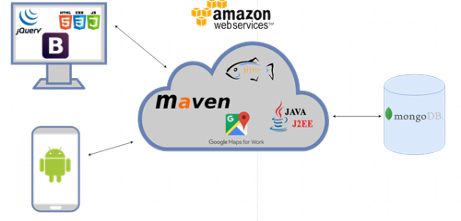
\includegraphics[width=0.9\textwidth]{images/architecture.png}
    \caption{System Architecture.}
    \label{image:sysArchitecture}
\end{figure}

Image \ref{image:sysArchitecture} can be referenced with the label given to the image, \\ i.e. \textbf{\textbackslash{}ref\{image:sysArchitecture\}}. Note that \LaTeX will place the image wherever it deems fit. Don't bother trying to change where a table or figure is placed until your document is ready for final layout.
\chapter{System Evaluation}
Evaluate your project against the objectives set out in the introduction.
This chapter should present results if applicable and discuss the strengths and weaknesses of your system. This is a clear opportunity for you to demonstrate your critical thinking in relation to the project. 


\section{Working with Tables}
Table \ref{table:HexToBin} can be referenced with the label given to the table, i.e. \textbf{\textbackslash{}ref\{table:HexToBin\}}. Note that \LaTeX will place the table wherever it deems fit. Don't bother trying to change where a table or figure is placed until your document is ready for final layout.

\begin{table}
    \begin{tabular}{p{2cm}|p{2cm}|p{2cm}|p{2cm}|p{2cm}|p{2cm}}
        \hline
        \multicolumn{6}{|c|}{Hexadecimal to Binary} \\
        \hline
        Hex & Binary 2 & Hex & Binary & Hex & Binary\\
        \hline
        \hline
        1 & 00000001 & B & 00001011 & 15 & 00010101 \\
        2 & 00000010 & C & 00001100 & 16 & 00010110 \\
        3 & 00000011 & D & 00001101 & 17 & 00010111 \\
        4 & 00000100 & E & 00001110 & 18 & 00011000 \\
        5 & 00000101 & F & 00001111 & 19 & 00011001 \\
        6 & 00000110 & 10 & 00010000 & 1A & 00011010 \\
        7 & 00000111 & 11 & 00010001 & 1B & 00011011 \\
        8 & 00001000 & 12 & 00010010 & 1C & 00011100 \\
        9 & 00001001 & 13 & 00010011 & 1D & 00011101 \\
        A & 00001010 & 14 & 00010100 & 1E & 00011110 \\
        \hline
    \end{tabular}
    \caption{Conversion from Hexadecimal to Binary}
    \label{table:HexToBin}
\end{table}
\chapter{Conclusion}
The significance of software development has increased significantly, and businesses heavily rely on applications to meet customer demands \cite{hf}. However, traditional development methods are no longer sufficient to meet the ever-increasing need for faster and more reliable software delivery \cite{sb}. Automation has emerged as a solution to tackle the problem of slow software development delivery. Continuous integration and continuous deployment (CI/CD) development practices have become increasingly popular for productivity and efficiency in recent years.

During this research, it became evident that Go, despite being initially considered easy to learn and use, can be quite challenging. Additionally, setting up CI/CD pipelines can be difficult, especially for those who are new to it or want to integrate an existing project. Different projects have to set up the pipeline in their way or according to different factors. However, the effort of setting up the pipelines is worth it, as it saves a lot of time when making changes to the code. CI/CD should be used more widely as it involves testing before deployment, which increases reliability.

The developer successfully incorporated a CI/CD pipeline into the project, meeting the objectives of the project. However, there is room for improvement in terms of planning and research in future projects. The use of tools like Jira can aid in better development planning and management, helping teams stay on track. Despite the need to recode the entire backend, the project was completed on time. To enhance the project's efficiency, it is crucial to consider the security of the database and take necessary measures to safeguard it against external threats. In summary, while the developer achieved the project's objectives, there is still room for improvement in terms of better planning and research for future projects, as well as enhancing the security of the database.

Overall, the adoption of continuous integration and continuous deployment (CI/CD) pipelines can greatly benefit organizations looking to streamline their software development processes \cite{kubinyi}. By automating the process of testing and deploying software, organizations can accelerate the development and delivery of software features, resulting in a shorter time-to-market, increased productivity, and a better overall customer experience \cite{kubinyi}. 

\section{Implications}
The adoption of continuous integration and continuous deployment pipelines can greatly improve the efficiency and effectiveness of software development processes. By automating the testing, deployment, and delivery of software, developers can reduce the risk of errors and ensure faster release cycles. This approach can also improve collaboration among development teams, operations, and other stakeholders, ultimately leading to better software quality and user satisfaction. More research or projects should be conducted to examine different aspects that will contribute to the CI/CD approach field so that developers and companies will be conscious of how it can affect software development processes.

\section{Limitations}
Despite the significant implications of this study, there were several limitations that must be acknowledged. First, the study was limited by the availability of data and resources. The developer did not have the final system written in GO for the backend due to this. Second, due to the time constraints of the project, the research focused on a limited number of CI/CD tools and practices. Finally, the study did not evaluate the long-term effectiveness of CI/CD pipelines, and additional research might need to determine the sustainability of these practices in the long run.

\section{Recommendations}
Researchers should aim to replicate this study in different contexts to determine the generalisability of the findings. Future studies should explore the effectiveness of a wider range of CI/CD tools and practices to determine the most effective approaches. Researchers should investigate the long-term effectiveness of CI/CD pipelines and evaluate their sustainability over time. Organizations that are considering the adoption of CI/CD pipelines should conduct a thorough analysis of their development environment, structure, and tools to ensure that they have the necessary resources and expertise to effectively implement these practices. Furthermore, project teams should consist of more than one person to ensure quality, and scope needs to be planned properly with efficient research to avoid encountering problems in the middle of the development process.


%------------------------------------------------------------------------------------------------------	
% Generate the bibliography. You may have to build the document more than once before all of the
% references and processed and cited correctly.
% WARNING: Don't mess with any of the following unless you know what you are doing.
%------------------------------------------------------------------------------------------------------	
\bibliographystyle{unsrt}
\bibliography{references.bib}

\appendix

\chapter{Jira}\label{appendix:jira}
\begin{figure}[h!]
    \centering
    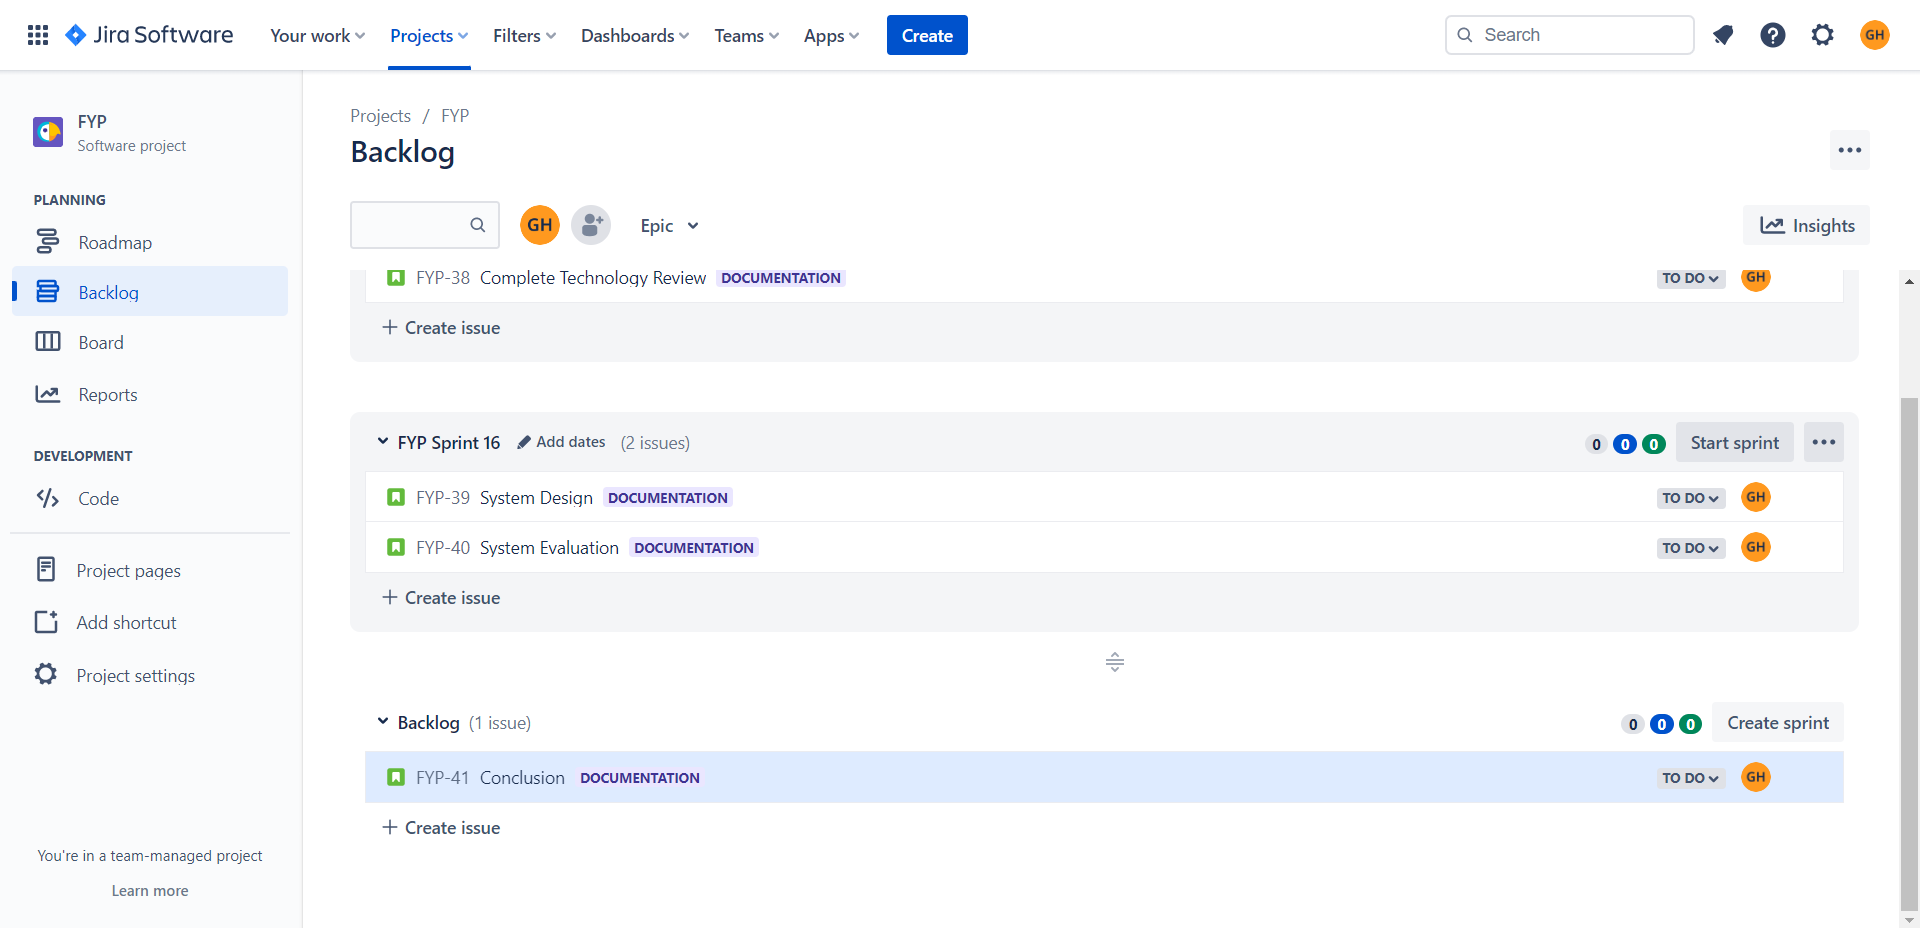
\includegraphics[width=0.9\textwidth]{images/backlog.png}
    \caption{Jira backlog}
    \label{image:backlog}
\end{figure}

\begin{figure}[h!]
    \centering
    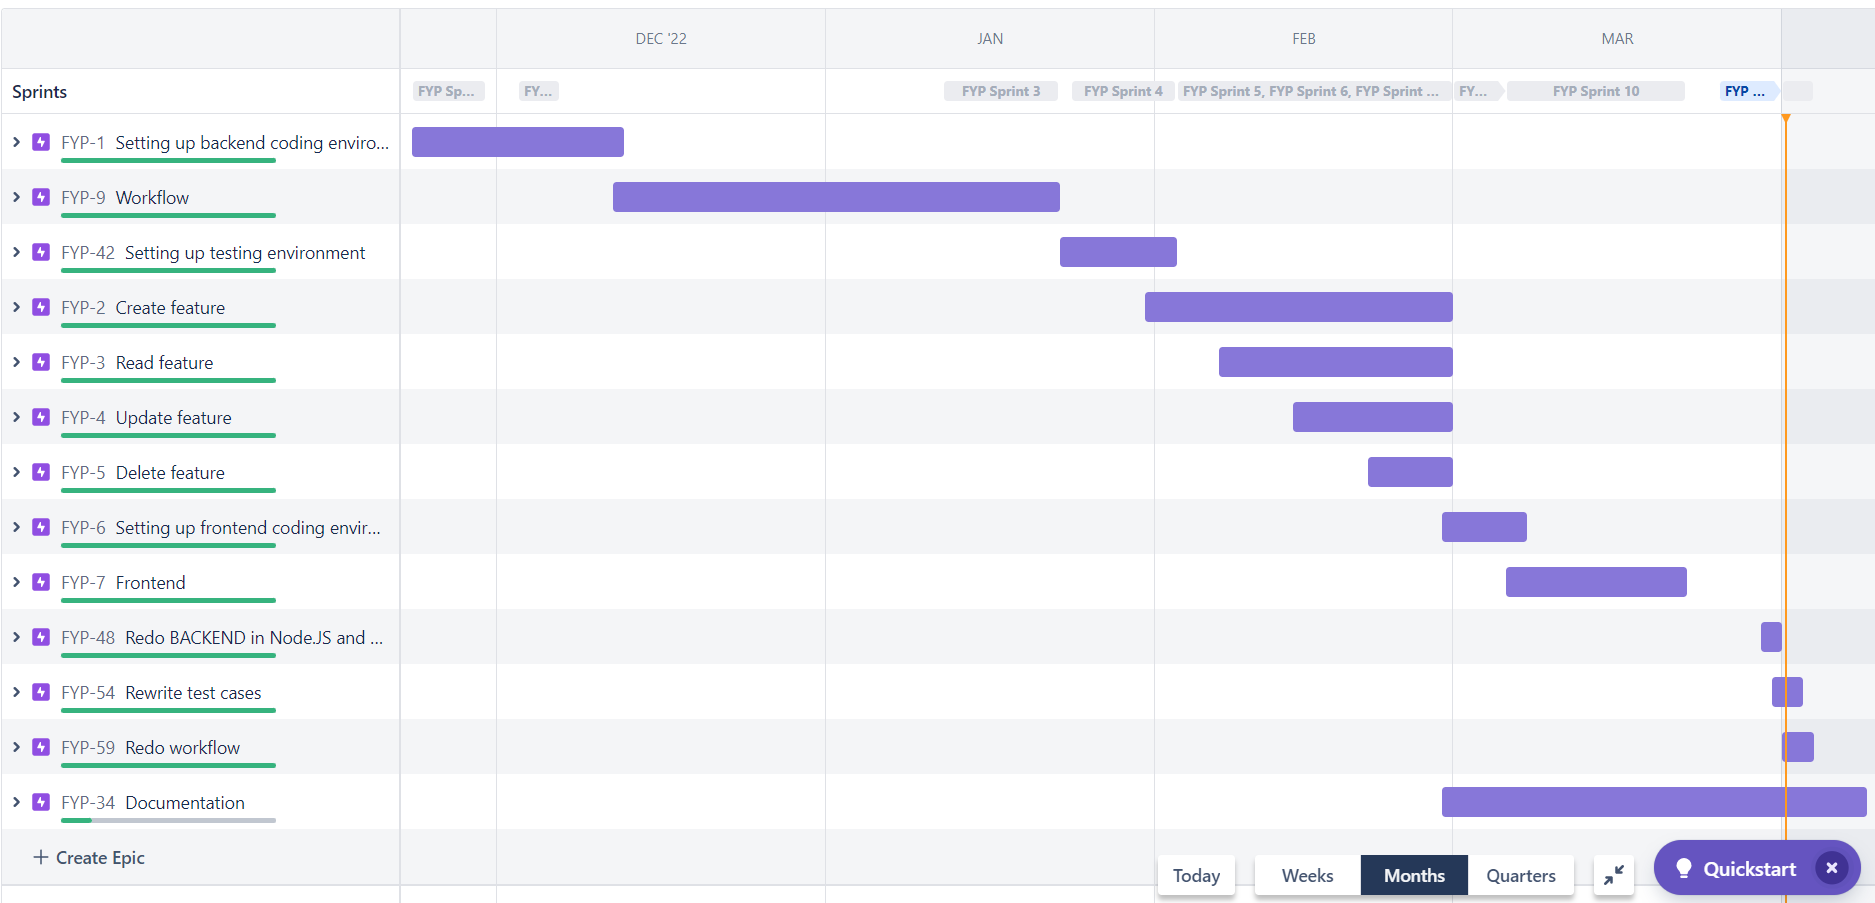
\includegraphics[width=0.9\textwidth]{images/roadmap.png}
    \caption{Jira roadmap}
    \label{image:roadmap}
\end{figure}

\begin{figure}[h!]
    \centering
    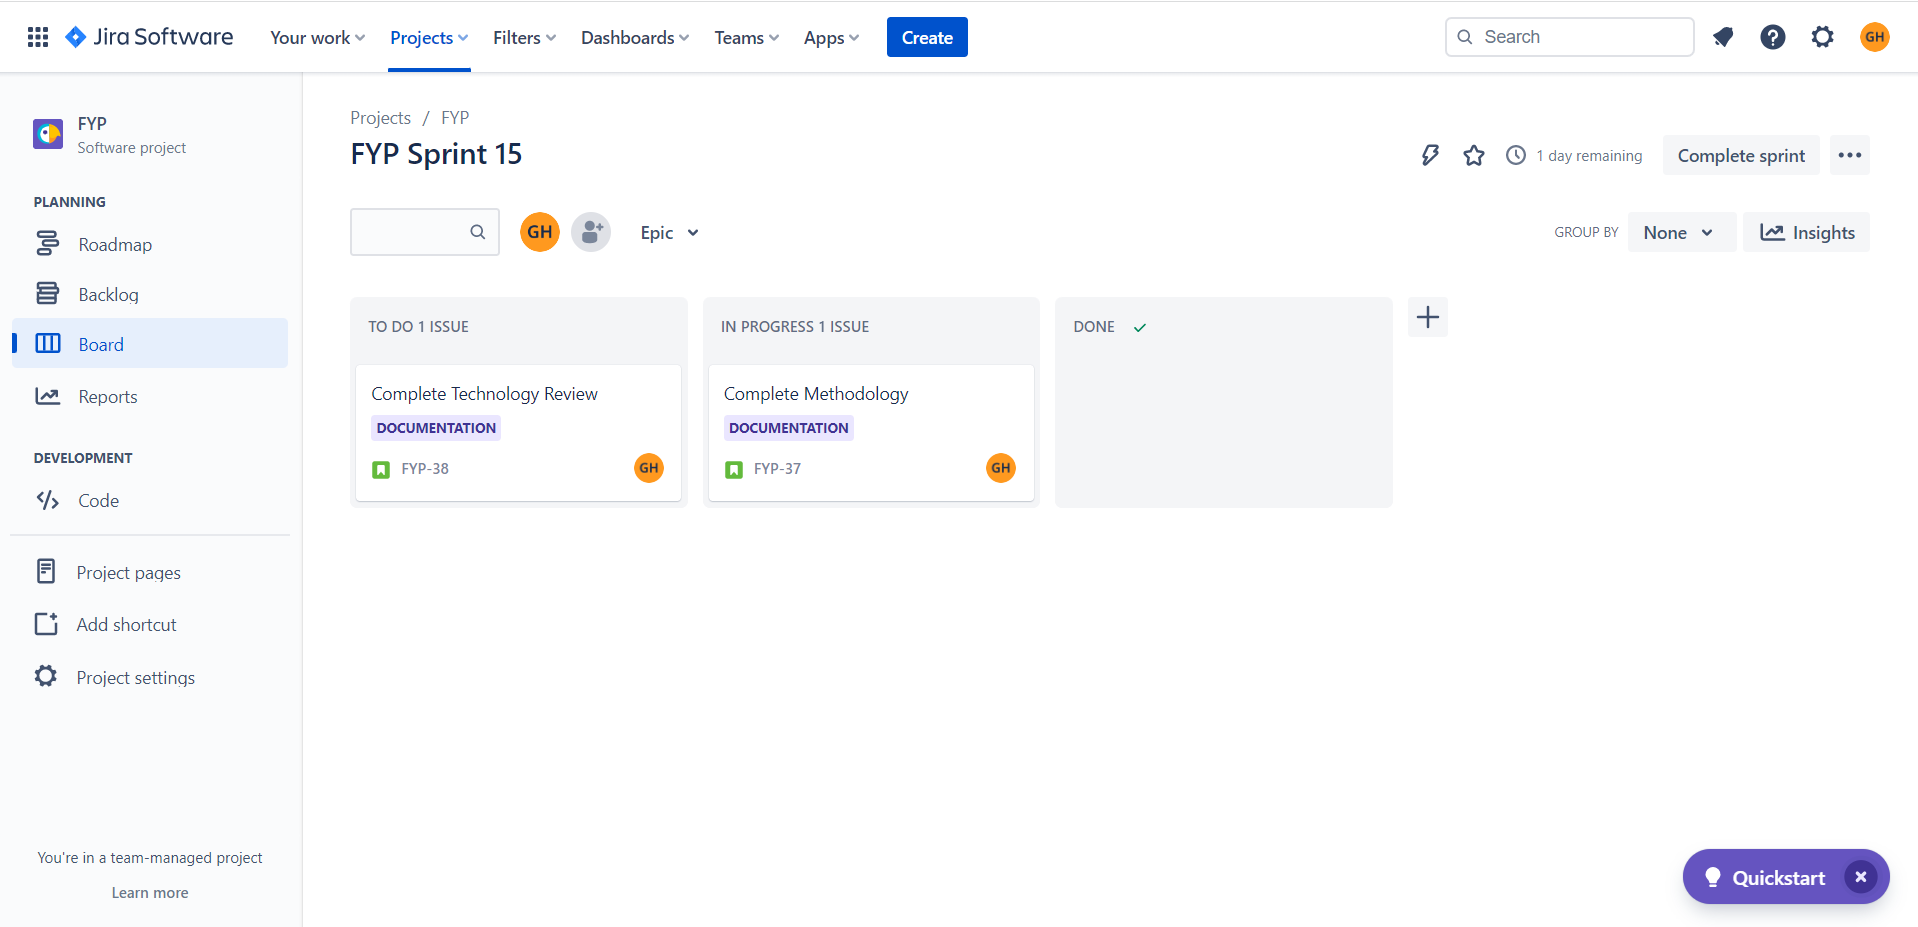
\includegraphics[width=0.9\textwidth]{images/board.png}
    \caption{Jira board}
    \label{image:board}
\end{figure}

\begin{figure}[h!]
    \centering
    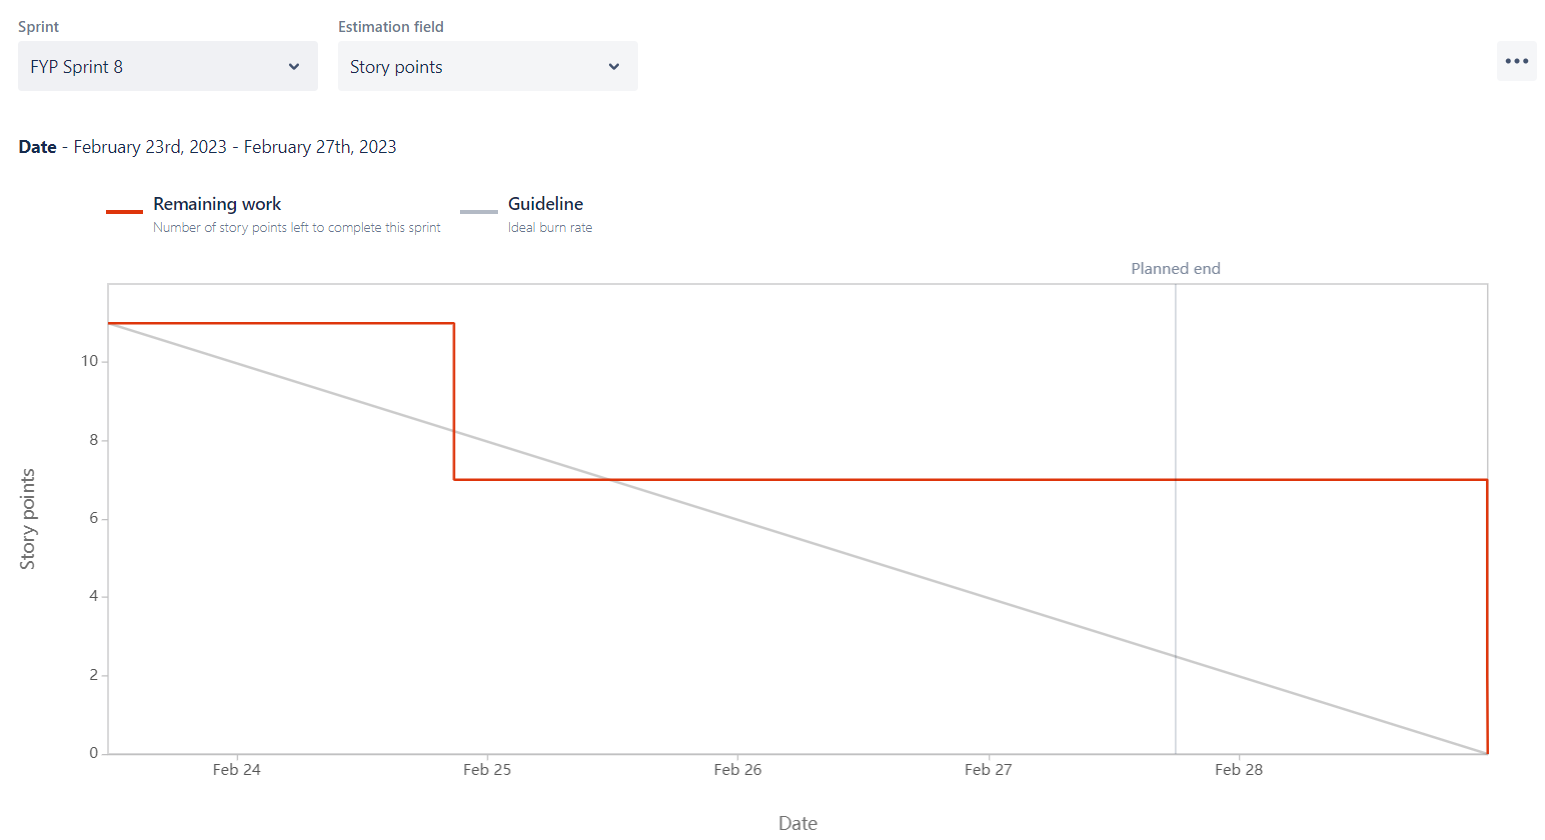
\includegraphics[width=0.9\textwidth]{images/sprint-burndown.png}
    \caption{A Sprint Burndown Chart}
    \label{image:sprint-burndown}
\end{figure}

\chapter{Scrum}\label{appendix:scrum}
\begin{figure}[h!]
    \centering
    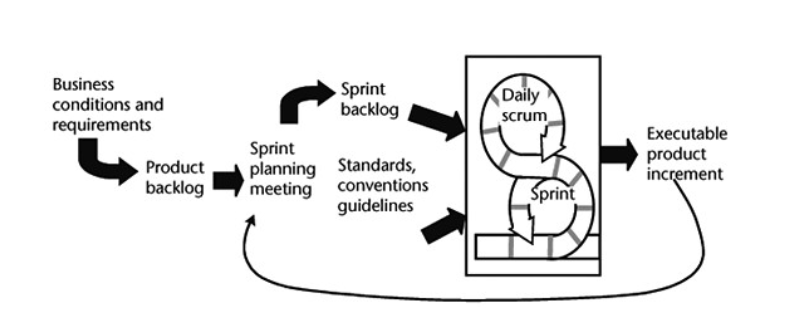
\includegraphics[width=0.9\textwidth]{images/scrum.png}
    \caption{Scrum Process Diagram}
    \label{image:scrum}
\end{figure}

\chapter{DevOps}\label{appendix:devops}
\begin{figure}[h!]
    \centering
    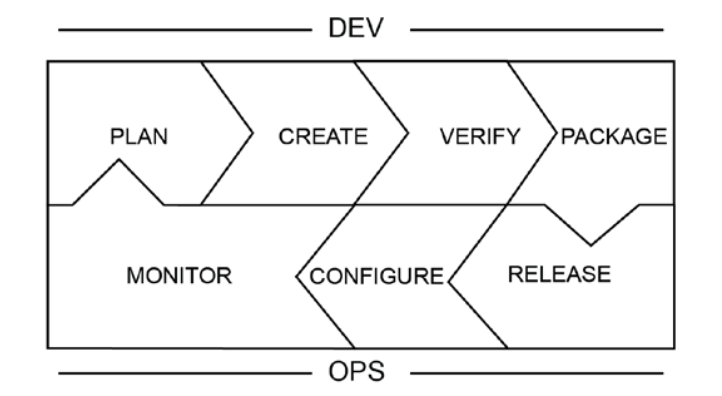
\includegraphics[width=0.9\textwidth]{images/devops.png}
    \caption{The DevOps Toolchain}
    \label{image:devops}
\end{figure}

\begin{figure}[h!]
    \centering
    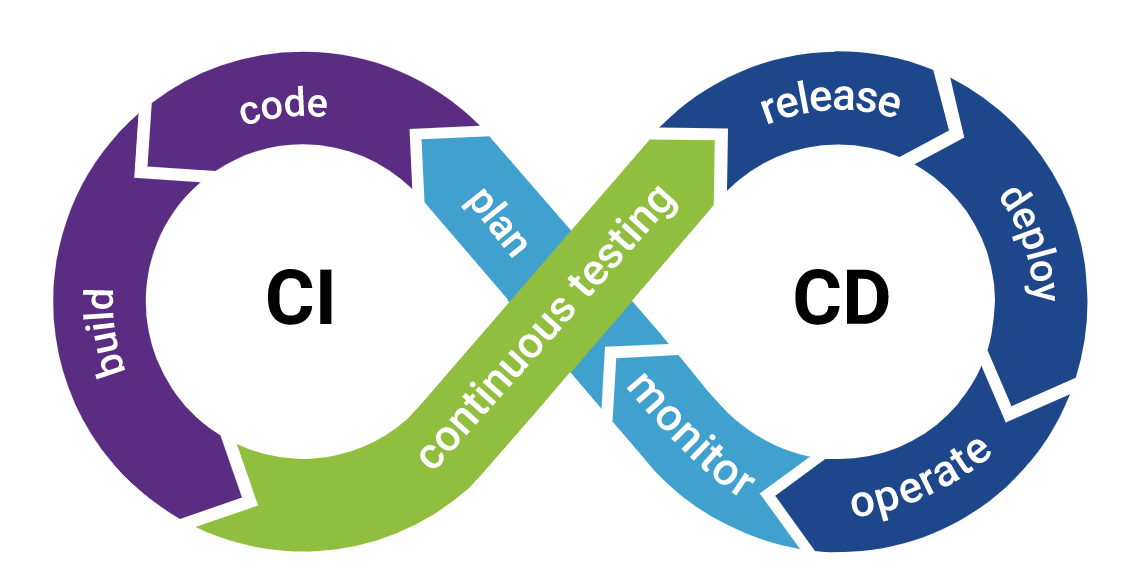
\includegraphics[width=0.9\textwidth]{images/CICD.png}
    \caption{The CI/CD Process}
    \label{image:cicd}
\end{figure}

\chapter{MERN}\label{appendix:mern}
\begin{itemize}
\item MongoDB: A database based on the document-oriented data model.
\item Express.js: A web application framework that allows for the creation of APIs and websites.
\item React.js: A JavaScript library for creating user interfaces that takes a declarative, component-based approach.
\item Node.js: A JavaScript runtime environment that enables the development of platform-independent servers, tools, and applications.
\end{itemize}

\begin{figure}[h!]
    \centering
    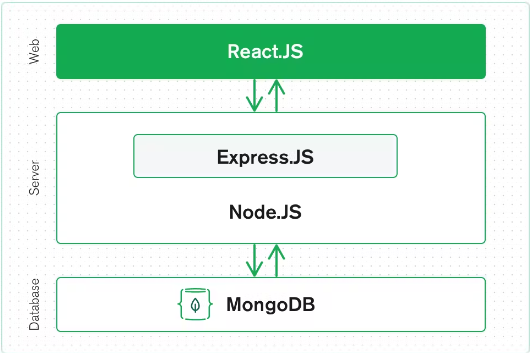
\includegraphics[width=0.9\textwidth]{images/mern.png}
    \caption{The MERN Stack Architecture}
    \label{image:mern}
\end{figure}

\chapter{CI/CD Design and Implementation}\label{appendix:CICD}
\begin{figure}[h!]
    \centering
    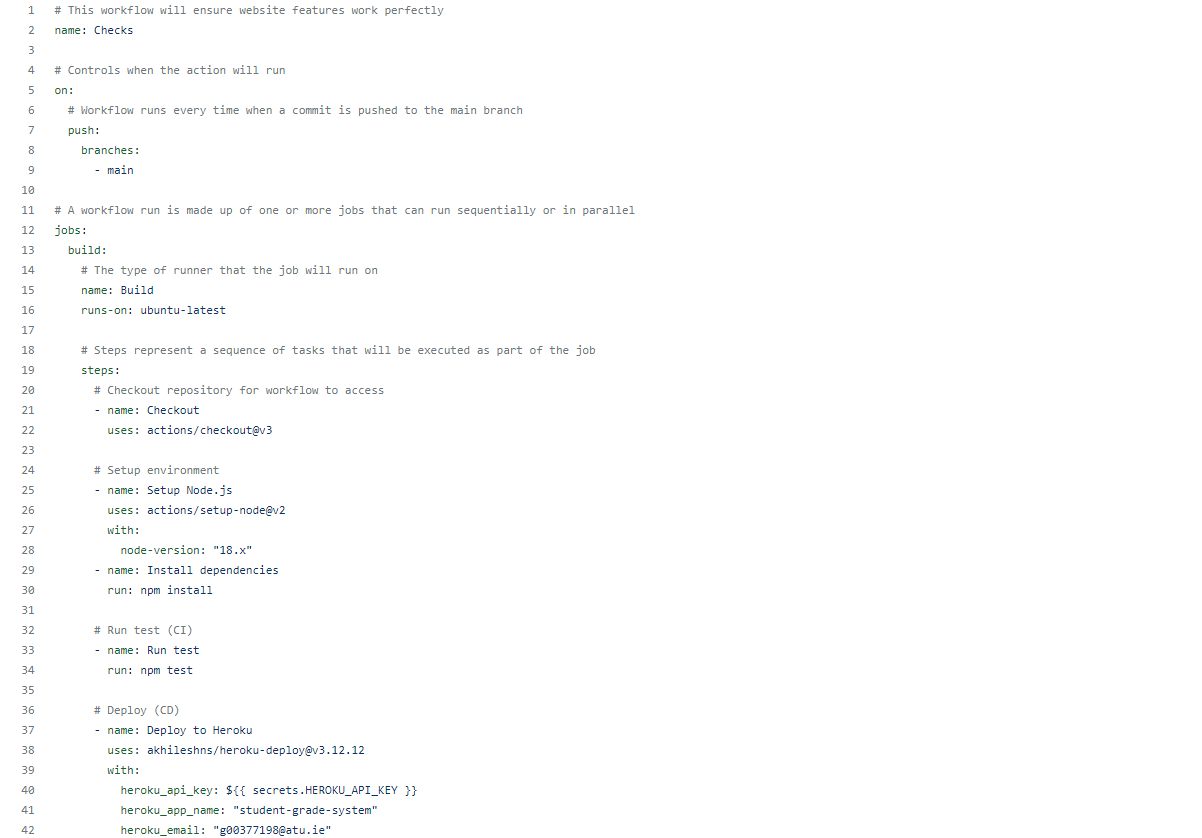
\includegraphics[width=0.9\textwidth]{images/full-workflow.png}
    \caption{GitHub Actions Workflow}
    \label{image:full-workflow}
\end{figure}

\begin{figure}[h!]
    \centering
    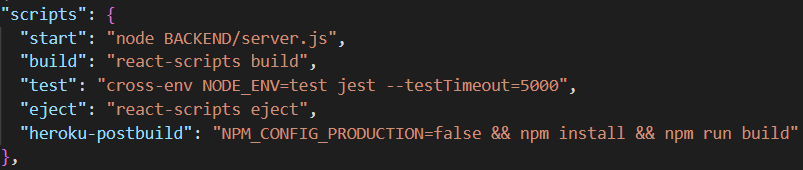
\includegraphics[width=0.9\textwidth]{images/heroku-build.png}
    \caption{Code Snippet from package.json to show heroku-postbuild}
    \label{image:heroku-build}
\end{figure}

\begin{figure}[h!]
    \centering
    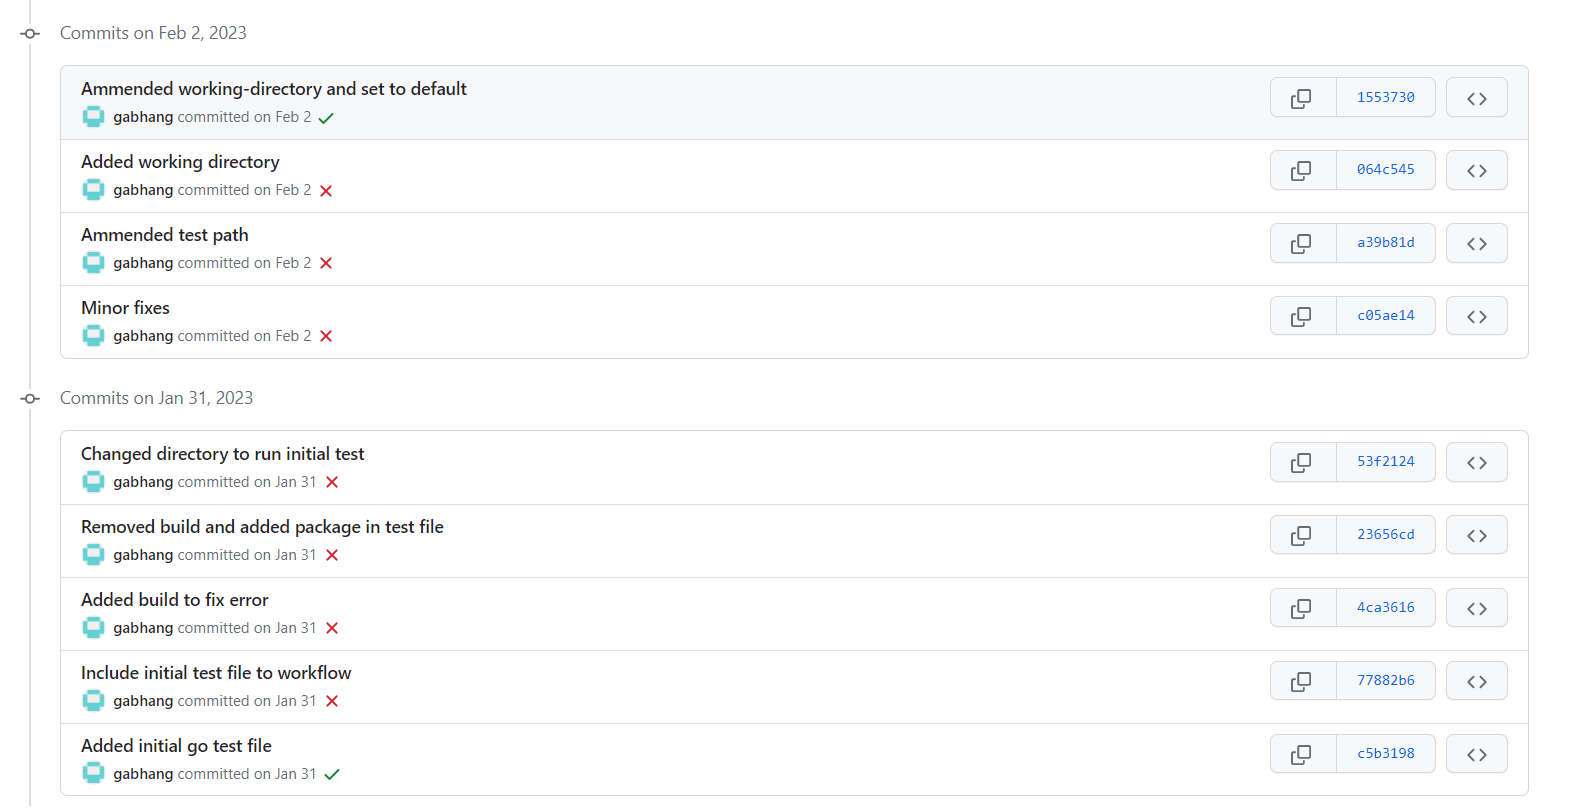
\includegraphics[width=0.9\textwidth]{images/workflow-failed.png}
    \caption{Evidence of mistakes and corrections during workflow design}
    \label{image:workflow-failed}
\end{figure}

\begin{figure}[h!]
    \centering
    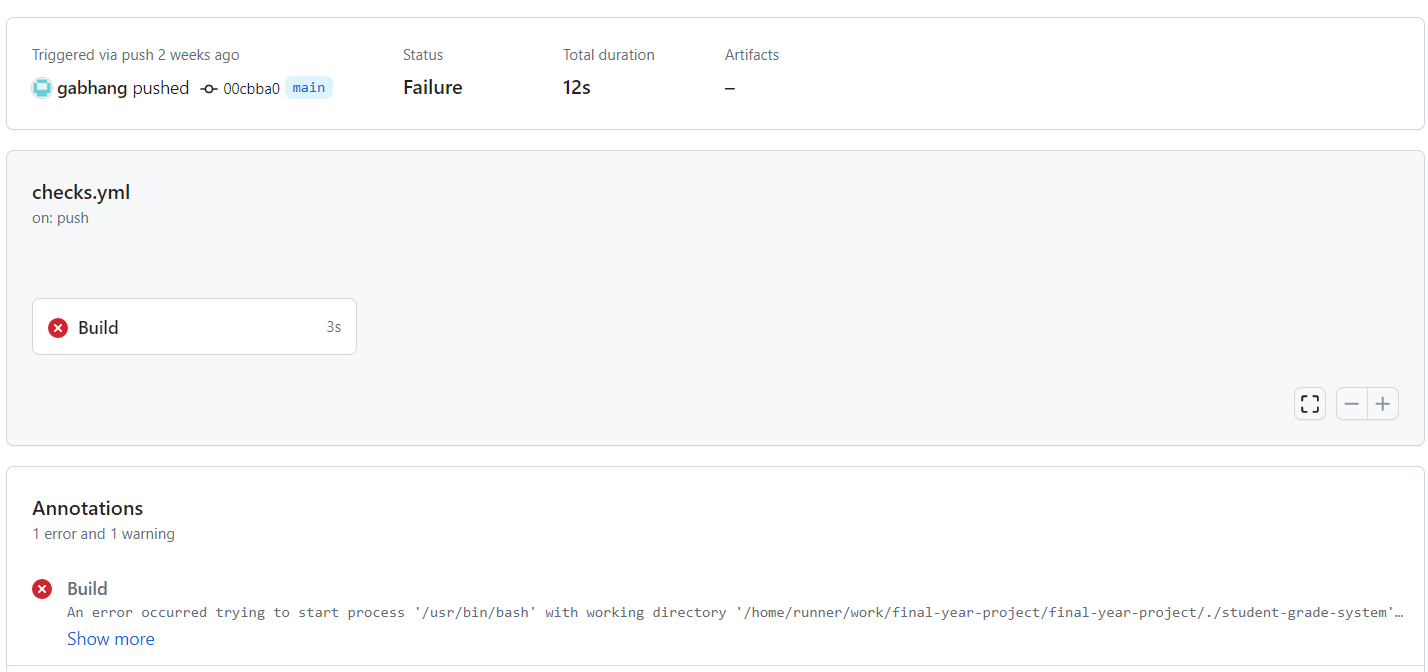
\includegraphics[width=0.9\textwidth]{images/build-fail-directory.png}
    \caption{Directory mismatch error}
    \label{image:build-fail-directory.png}
\end{figure}

\begin{figure}[h!]
    \centering
    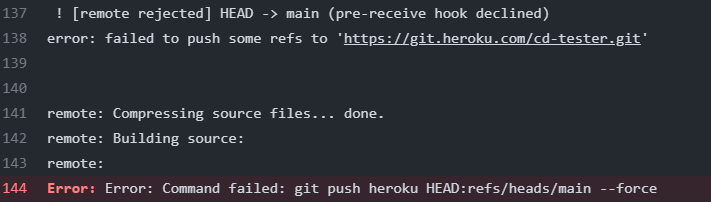
\includegraphics[width=0.9\textwidth]{images/heroku-go-issue.png}
    \caption{Deployment rejection from using GO}
    \label{image:heroku-go-issue.png}
\end{figure}

\begin{figure}[h!]
    \centering
    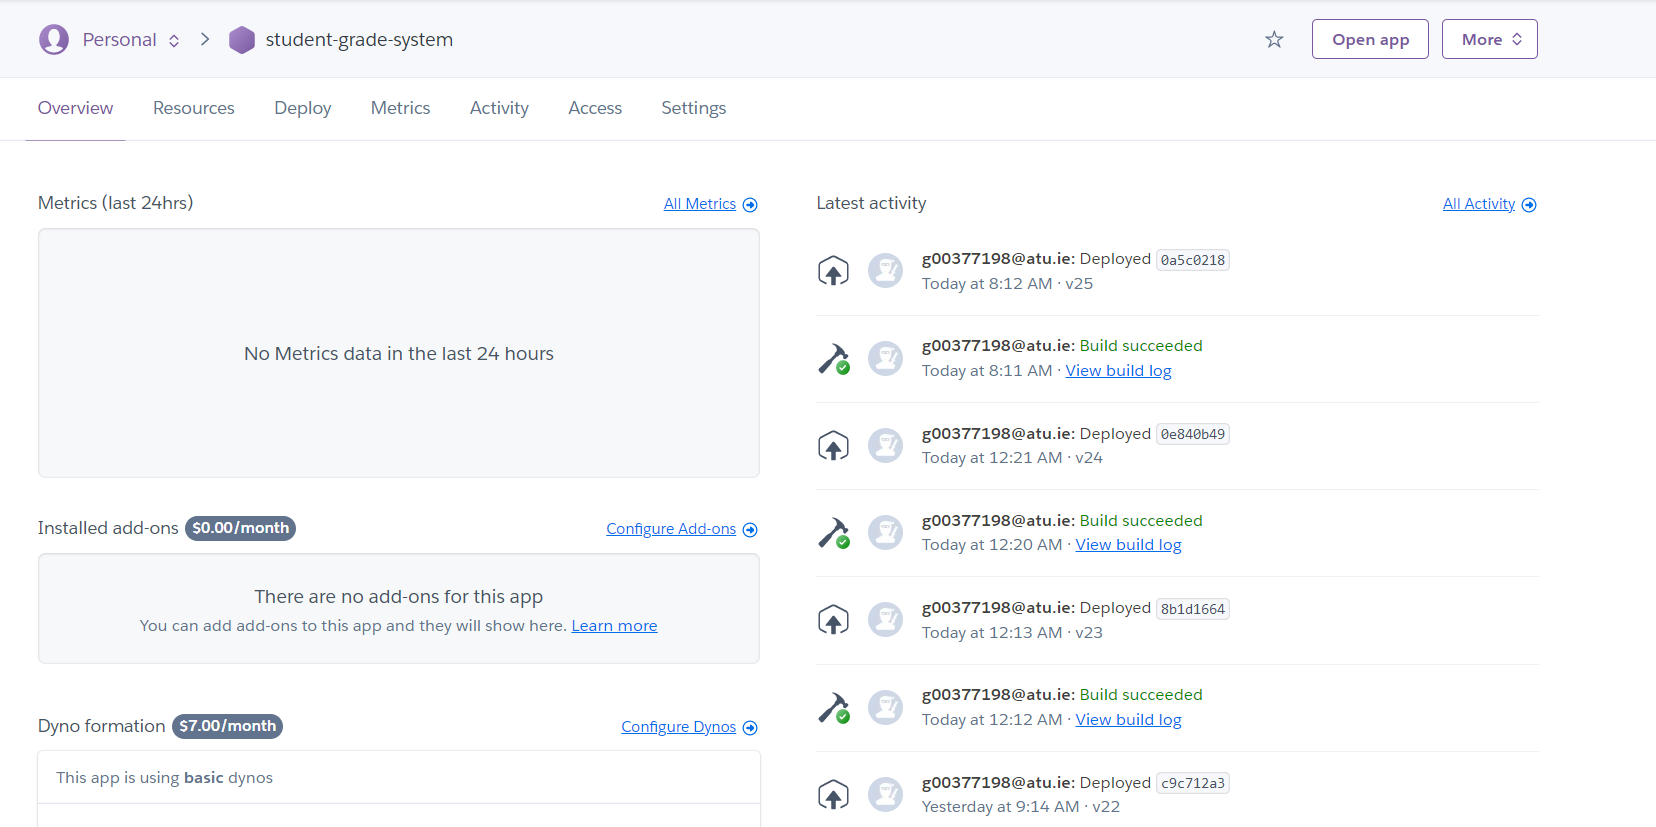
\includegraphics[width=0.9\textwidth]{images/heroku-success.png}
    \caption{Successful deployment in Heroku}
    \label{image:heroku-success.png}
\end{figure}
\end{document}